\documentclass[11pt, letterpaper]{article}
\usepackage[utf8]{inputenc}
\usepackage[letterpaper, margin=0.5in]{geometry}
\usepackage{amsmath}
\usepackage{amssymb}
\usepackage{amsthm}
\usepackage{graphicx}
\usepackage[font=scriptsize]{caption}
\usepackage{subcaption}
\graphicspath{ {.} }
\captionsetup{justification=raggedright, singlelinecheck=false}


\title{STA 602 HW2}
\author{Ryan Tang}
\date{September 11th 2022}

\begin{document}
\maketitle

\section{Excerise 3.1}
\paragraph{(a)}
\begin{align*}
    Y_{i\in N} \overset{iid}{\thicksim} Bernoulli(\theta) && N &= 100 \\
    p(y_1, y_2 \dots y_{100}) &= \prod_{i=1}^{100} \mathbb{I}(y_i=1)\theta + \mathbb{I}(y_i=0)(1-\theta) \\
        &= {\theta^{N_1}(1-\theta)}^{N_0} && N_1 = \sum_{i=1}^{100} \mathbb{I}(y_i=1) \\
    p(\sum_i^{100} y_i | \theta) &= \binom{100}{N_1} {\theta^{N_1}(1-\theta)}^{N_0}
\end{align*}

\paragraph{(b) $\thicksim$ (e)}

\begin{figure*}[!b]
    \centering
    \begin{subfigure}{.49\textwidth}
        \centering
        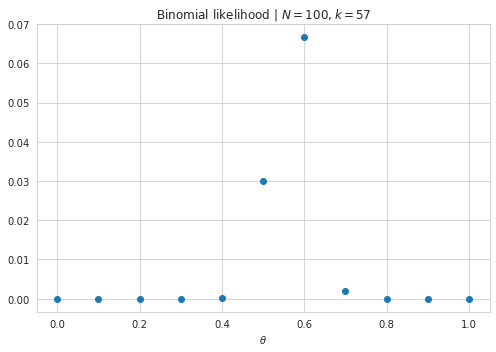
\includegraphics[scale=0.44]{hw2_binom1.png}
        \caption{plot for 3.1.b --- Likelihood Distribution $p(\mathbf{x}=57|\theta, n=100)$}
    \end{subfigure} %    
    \begin{subfigure}{.49\textwidth}
        \centering
        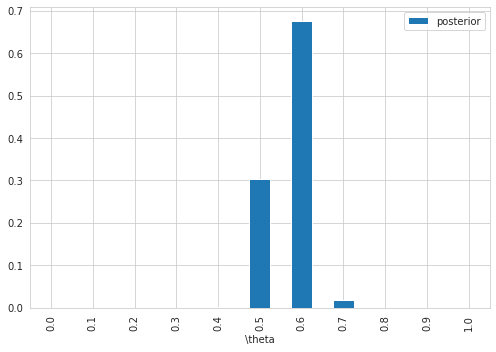
\includegraphics[scale=0.44]{hw2_binom_post1.png}
        \caption{plot for 3.1.c --- Posterior Distribution $p(\theta|\mathbf{x})$}
    \end{subfigure}
    \begin{subfigure}{.49\textwidth}
        \centering
        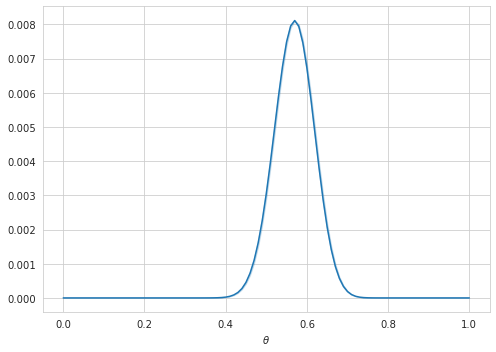
\includegraphics[scale=0.44]{hw2_3.1.d.png}
        \caption{plot for 3.1.d --- Posterior Distribution $p(\theta|\mathbf{x})$ on continuous Uniform prior}
    \end{subfigure}
    \begin{subfigure}{.49\textwidth}
        \centering
        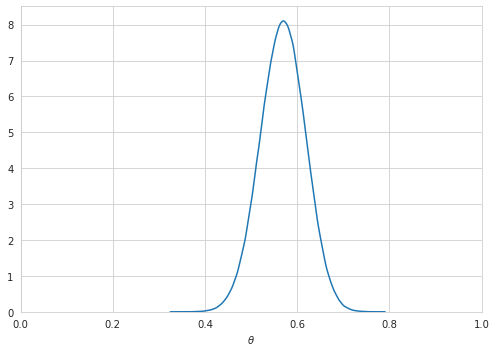
\includegraphics[scale=0.44]{hw2_3.1.e.png}
        \caption{plot for 3.1.d --- $Beta(58, 44)$ Density}
    \end{subfigure}
\end{figure*}

To summarize below, all 4 plots, (a) and (b), are just the coalesced version for Bayesian belief updates. (c) shows the posterior
after applying to the Uniform prior. Lastly, (e) confirms that the Beta distribution is conjugate to the Binomial likelihood, and
the Uniform prior, equivalent to a $Beta (1, 1)$ distribution, has been treated as a weak prior belief with only 2 sample sizes.
Hence, the resulting posterior is also a Beta distribution.


\section{Excerise 3.2}
Figure 2 shows the sensitivity analysis on how various prior beliefs would affect the resulting posterior belief after
observing the survey data, $N=100, \sum y_i = 57$.
\begin{itemize}
    \item If one has a strong prior belief, top right corner, it is hard to move the prior without significant evidence.
    \item On the contrary, suppose one does not hold a strong belief, bottom left corner, he or she should take the survey evidence strongly.
\end{itemize}

\begin{figure}[h]
    \centering
    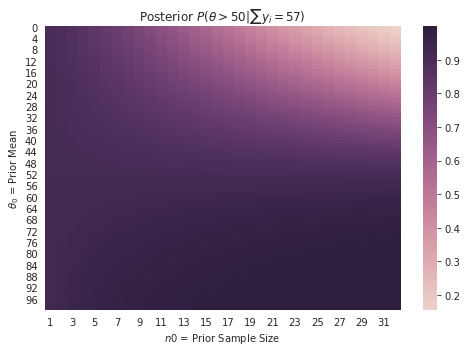
\includegraphics[width=0.5\textwidth]{hw2_3.2.png}
    \caption{Posterior Sensitivity}
\end{figure}


\section{Excerise 3.4}
\paragraph{(a)}
Using the $Beta(2, 8)$ prior, and the survey data $N = 43, k = 15$, we shall obtain the following posterior.
Mode = 0.31, Mean = 0.32,  and the standard deviation = 0.0635.
The 95$\%$ confidence interval of the parameter $\hat{\theta} \in [0.2, 0.44]$.

\begin{figure}[h]
    \captionsetup{justification=centering, margin=2cm}
    \centering
    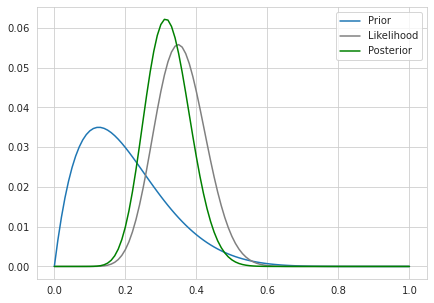
\includegraphics[width=0.5\textwidth]{hw2_3.4.png}
    \caption{Bayes Updates Demonstration}
\end{figure}

\paragraph{(b)}
If we are using the $Beta(8, 2)$ prior, we shall obtain the following posterior instead.
Mode = 0.43, Mean = 0.434,  and the standard deviation = 0.0674.
The 95$\%$ confidence interval of the parameter $\hat{\theta} \in [0.3, 0.56]$.

\begin{figure}[h]
    \captionsetup{justification=centering, margin=2cm}
    \centering
    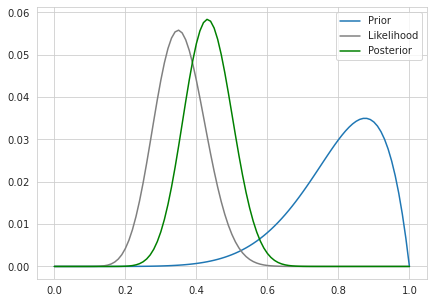
\includegraphics[width=0.5\textwidth]{hw2_3.4.b.png}
    \caption{Bayes Updates Demonstration}
\end{figure}

\paragraph{(c)}
Here we are considering a mixture of two beta distributions, and Figure 5 compares the three distributions.
The new mixture can be considered as we think there are two latent cohorts within the population.
One cohort has a much lower chance of re-offending than the other.

\begin{figure}[h]
    \captionsetup{justification=centering, margin=2cm}
    \centering
    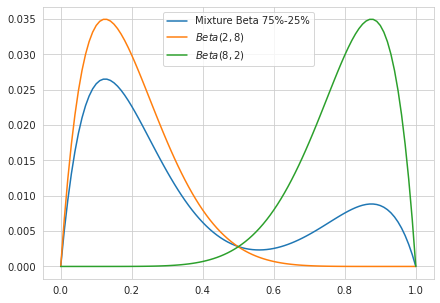
\includegraphics[width=0.5\textwidth]{hw2_3.4.c.png}
    \caption{Prior comparisons}
\end{figure}

\paragraph{(d)}
If we start using the Beta mixture prior to the Binomial likelihood, the posterior can be derived as follow.
\begin{align*}
    p(\theta) &= \frac{1}{4}\frac{\Gamma(10)}{\Gamma(2)\Gamma(8)}[3\theta{(1-\theta)}^7+\theta^7(1-\theta)] \\
    p(\theta|y) &\propto p(y|\theta)p(\theta) \\
        &= \frac{1}{4}\frac{\Gamma(10)}{\Gamma(2)\Gamma(8)}[3\theta{(1-\theta)}^7+\theta^7(1-\theta)] \binom{43}{15}\theta^{15}{(1-\theta)}^{28} \\
        &\propto [3\theta{(1-\theta)}^7+\theta^7(1-\theta)] \theta^{15}{(1-\theta)}^{28} \\
        &= \frac{3}{4}[\theta^{17-1}{(1-\theta)}^{36-1}] + \frac{1}{4}[\theta^{23-1}{(1-\theta)}^{30-1}] \\
        &= 75\% \cdot Beta(17, 36) + 25\% \cdot Beta(23, 30)
\end{align*}
Therefore, the resulting posterior is still a Beta distribution, although it is in its mixture form.
Furthermore, the posterior distribution is plotted below in Figure 6.

\begin{figure}[h]
    \captionsetup{justification=centering, margin=2cm}
    \centering
    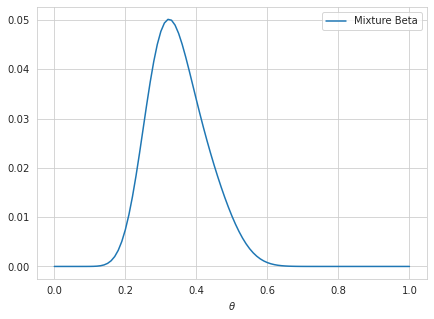
\includegraphics[width=0.5\textwidth]{hw2_3.4.d.png}
    \caption{Posterior Distribution from the Beta Mixture Prior of $75\% \cdot Beta(2, 8) + 25\% \cdot Beta(8, 2)$}
\end{figure}

It has a Mode = 0.32, which is very close to the $Beta(2, 8)$ distribution. In other words, the evidence is 
strong enough to overwrite the bi-modality and favors one of the modes based on the prior beliefs.

\paragraph{(e)}
As derived in (d), the Beta mixture has a general form of following, which is simply a weighted sum.
\[
    p(\theta|a_1, a_2, b_1, b_2, w_1) = w_1\cdot Beta(a_1, b_1) + (1-w_1) \cdot Beta(a_2, b_2)
\]


\section{Excerise 3.7}
\paragraph{(a)}
Given the Uniform prior or $Beta(1, 1)$ and Binomial likelihood. The survey data with $N = 15, k = 2$ results in
$Beta(3, 14)$ posterior. Hence, it has mean 0.176, mode 0.133, and standard deviation 0.08985.

\begin{figure}[h]
    \captionsetup{justification=centering, margin=2cm}
    \centering
    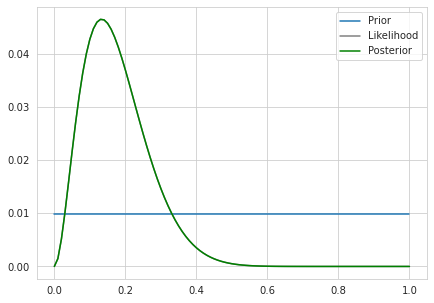
\includegraphics[width=0.5\textwidth]{hw2_3.7.png}
    \caption{First survey posterior with an Uniform prior}
\end{figure}

\paragraph{(b)}
For the joint and the predictive posterior distribution to be true, we assume $Y_2$ comes from the same population
as $Y_1$ and the underlying generative process is the same as $Y_1$, that is, $iid$. So that our $theta$ posterior
is appliable. In order to make an inference, we also need to assume that the likelihood function is known,
for instance, Binomial in this case.

Plugging both pdfs we arrive at a BetaBinomial for the posterior predictive distribution.
\begin{align*}
    p(y_2|y_1=2) &= \int_0^1{p(y_2|\theta, y_1=2)p(\theta|y_1=2)} \, d\theta  \\
      &= \int_0^1 \binom{278}{y_2} \theta^{y_2} {(1-\theta)}^{278-y_2} {\mathbf{B}(3, 14)}^{-1}\theta^2{(1-\theta)}^{13} \, d\theta \\
      &= \binom{278}{y_2} {\mathbf{B}(3, 14)}^{-1} \int_0^1 \theta^{y_2+2} {(1-\theta)}^{291-y_2} \, d\theta \\
      &= \binom{278}{y_2} \frac{\mathbf{B}(y_2+3, 278+14-y_2)}{\mathbf{B}(3, 14)} \\
      &\thicksim BetaBinomial(y_2 | n=278, \alpha = 3, \beta = 14)
\end{align*}

\paragraph{(c)}
The resulting posterior predictive distribution has a mean of 49.05 and a standard deviation of 25.73.

\begin{figure}[h]
    \captionsetup{justification=centering, margin=2cm}
    \centering
    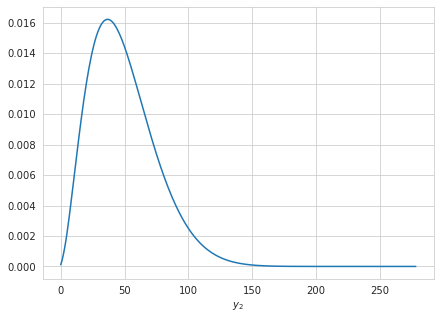
\includegraphics[width=0.5\textwidth]{hw2_3.7.c.png}
    \caption{Posterior Predictive Distribution --- BetaBinomial}
\end{figure}

\paragraph{(d)}
Suppose we use MLE to estimate the latent variable $\theta$. We arrive at the $2/15$, which is the mode of our posterior
from (a) --- MAP results. Figure 9.

\begin{figure}[!h]
    \captionsetup{justification=centering, margin=2cm}
    \centering
    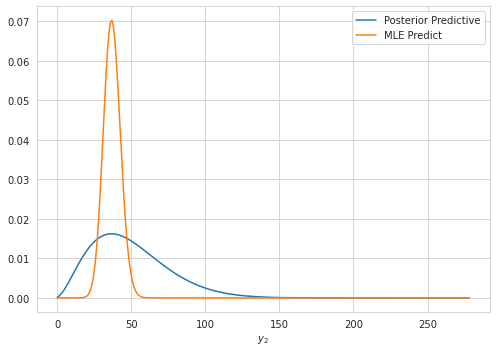
\includegraphics[width=0.5\textwidth]{hw2_3.7.d.png}
    \caption{Posterior Predictive vs. MLE}
\end{figure}

Usually, a frequentist would use the estimate in Binomial to arrive at the prediction. The comparisons
are plotted below with the bayesian approach. MLE can underestimate the uncertainty at several magnitudes; in
other words, it does not consider the sample size uncertainty from Survey 1. On the contrary, posterior predictive distribution
takes into account all of it.


\section{Excerise 3.10}
\paragraph{(a)}
\begin{align*}
    \psi &= \log[\theta/(1-\theta)] = g(\theta) && where \, \theta \thicksim Beta(a, b) \\
    e^{\psi} &= \frac{\theta}{(1- \theta)} \\
    \theta &= \frac{e^{\psi}}{1+e^{\psi}} = 1 - \frac{1}{1+e^{\psi}} = g^{-1}(\psi)
\end{align*}

With the inverse transformation function, we can derive the density function for $\psi$.
\begin{align*}
    p(\psi) &= p_{\theta}(g^{-1}(\psi)) \cdot \mid \frac{\partial g^{-1}}{\partial \psi} \mid \\
      &= p_{\theta}(1 - \frac{1}{1+e^{\psi}}) e^{\psi} {(1+e^{\psi})}^{-2} \\
      &= {\mathbf{B}(a, b)}^{-1} {(1 - \frac{1}{1+e^{\psi}})}^{a-1} {(\frac{1}{1+e^{\psi}})}^{b-1} e^{\psi} {(1+e^{\psi})}^{-2} \\
      &= {\mathbf{B}(a, b)}^{-1} {(1 - \frac{1}{1+e^{\psi}})}^a {(\frac{1}{1+e^{\psi}})}^b
\end{align*}

\begin{figure}[h]
    \captionsetup{justification=centering, margin=2cm}
    \centering
    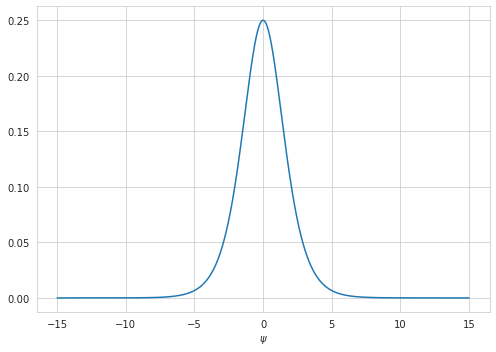
\includegraphics[width=0.5\textwidth]{hw2_3.10.a.png}
    \caption{The distribution of $\psi = \log[\theta/(1-\theta)]|a = b = 1$}
\end{figure}

\vspace{3in}

\paragraph{(b)}
\begin{align*}
    \psi &= \log[\theta] = g(\theta) && where \, \theta \thicksim Gamma(a, b) \\
    e^{\psi} &= \theta = g^{-1}(\psi)
\end{align*}

With the inverse transformation function, we can derive the density function for $\psi$.
\begin{align*}
    p(\psi) &= p_{\theta}(g^{-1}(\psi)) \cdot \mid \frac{\partial g^{-1}}{\partial \psi} \mid \\
      &= \frac{b^a}{\Gamma(a)} e^{\psi(a-1)} e^{-be^{\psi}} e^{\psi} \\
      &= \frac{b^a}{\Gamma(a)} e^{a\psi} e^{-be^{\psi}}
\end{align*}

\begin{figure}[h]
    \captionsetup{justification=centering, margin=2cm}
    \centering
    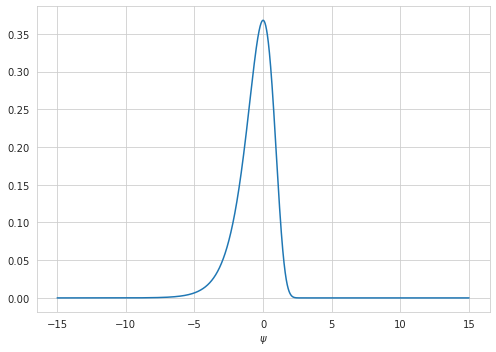
\includegraphics[width=0.5\textwidth]{hw2_3.10.b.png}
    \caption{The distribution of $\psi = \log[\theta]|a = b = 1$}
\end{figure}

\end{document}